%!TEX root = ../thesis.tex
\chapter{Trading Model}
\label{chap:trading model}

Our trading model is pairs trading model. Pairs are constructed from cointegrated stocks in SP500 stocks in function training\_model(). Then, each pairs is to implement bollinger band strategy in function building\_model(). Later, our trading model will enter function backtesting() with trading signals and corresponding PnL.

\section{Training}

\subsection{Parameters}
\begin{itemize}
    \item training start date: 2014-01-01, training end date: 2018-01-01
    \item capital: 1,000,000 for each pair
    \item cointegration: significance = 0.05
    \item Bollinger Band: standard deviation = 2, moving average period = 10
    \item PCA: principle components = 50, epsilon = 1.8, minimum sample = 3
\end{itemize}

\subsection{Steps}
\begin{enumerate}
    \item 500 stocks price return data of 4 years are reduced to 50 principle components using PCA (background in Section 2.2.1). The resulting dataframe is then in 50 * 500 dimension.
    \item We apply DBSCAN Clustering (background in 2.2.2) to group stocks according to 50 principle components. It will result in 6 to 10 groups with minimum of 3 stocks per group.
    \item Pairs are selected within each group. In each group, every two stocks go through cointegration test (background in 2.1.1). As shown in Figure 4.1, only pairs that pass the test most significantly (smallest p-value, or largest t-statistics) in each group are selected. Information about pairs are stored in table "stockpairs". As shown in Figure 4.2, all pairs have large score (t-statistics).
    \item We then regress one stock price series to another stock price series for each pair using training data. Residual is then constructed in this way as in Equation (2.4). Later, we build bollinger band using residuals (background in Section 2.1.2). Pairs prices, residuals and bollinger bands data are stored in table "pairprices". 
\end{enumerate}

\begin{figure}
\centering
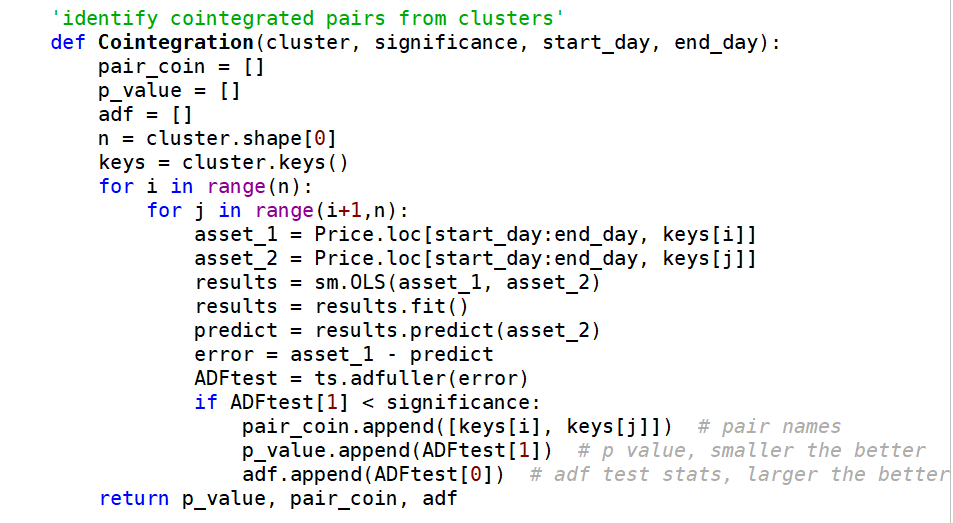
\includegraphics[scale=0.6]{model/images/cointegration.png}
\caption{Function: Cointegration()}
\label{fig:cointegration}
\end{figure}

\begin{figure}[h!]
\centering
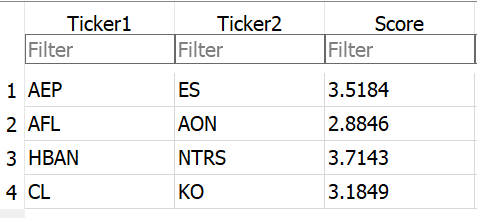
\includegraphics[scale=0.8]{model/images/stockpairs.png}
\caption{Table: Stockpairs}
\label{fig:stockpairs}
\end{figure}




\section{Backtesting}

We backtest from 2018-01-01 to 2019-01-01 for one year. A class is constructed for each stock pair shown in Figure 4.3, where trade is created with stock pair data of each day and is updated if there is a trading signal. Each pair is assigned with equal capital and is market neutral. Profit and loss is also calculated daily according current position and price. Backtesting result is stored in table "trades".


\begin{figure}[h!]
\centering
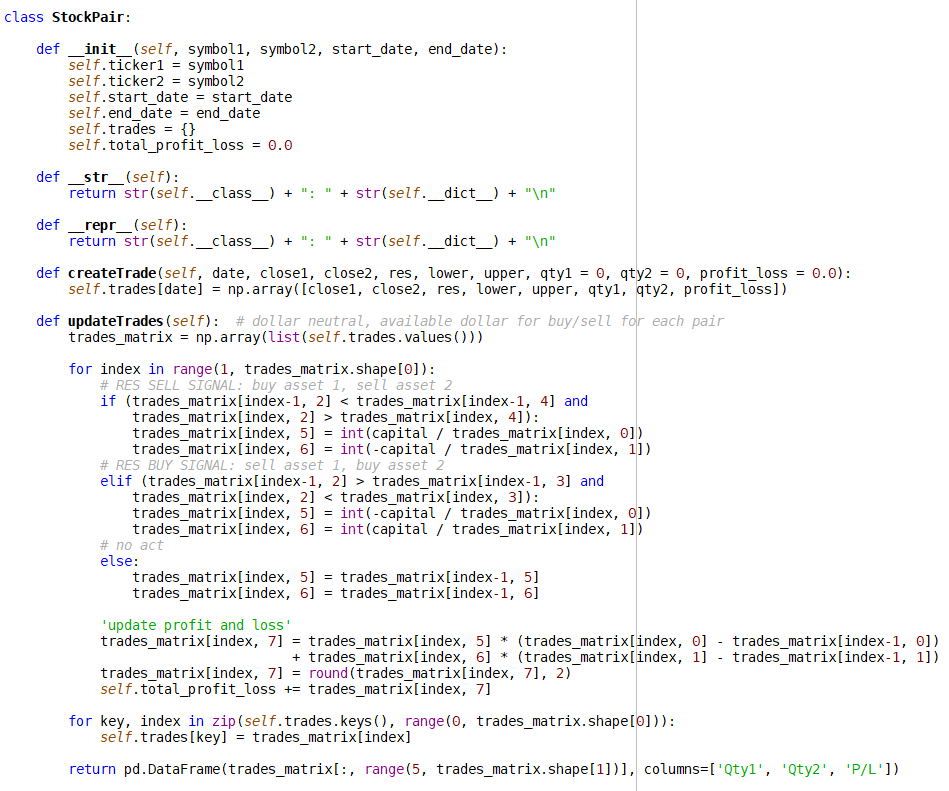
\includegraphics[scale=0.8]{model/images/class.png}
\caption{Class: StockPair}
\label{fig:class}
\end{figure}

